\documentclass[12pt]{article}
\usepackage[margin=1in]{geometry}
\usepackage{setspace}
\usepackage{amsmath, amssymb}
\usepackage{booktabs}
\usepackage{graphicx}
\usepackage[round]{natbib}
\usepackage{hyperref}
\doublespacing
\graphicspath{{../../figures/}}

\title{Lattice-Reduction Attack as a Pipeline Stage:\\
v8 --- Why Conflict Learning and Kernel Enumeration Failed,\\
and What the AHL Embedding Delivers}
\author{neuroMCTS project}
\date{July 2026}

\begin{document}
\maketitle

\begin{abstract}
Following the agreed roadmap, three search technologies were implemented and compared on a fixed benchmark of sixty hard $20 \times 50$ instances that the v7 pipeline could not close (forty unsolved feasible, twenty unproven infeasible). Conflict-directed backjumping with reason tracking and activity-based dynamic ordering --- verified exhaustively on 300 small instances --- closed \emph{none} of them within 500{,}000 nodes, performing identically to chronological DFS: on rows of density one half, conflict reasons span nearly all decisions and backjumping degenerates. Enumeration in the LLL-reduced integer kernel lattice (built from a column Hermite normal form with recorded unimodular transform, least-squares recentering, and provably valid coefficient boxes) closed two of the forty feasible instances; dynamic per-node bounds added cost without pruning power. The Aardal--Hurkens--Lenstra-style solution embedding, by contrast, lets BKZ reduction reveal verified 0/1 solutions directly: 19 of the 40 hard feasible instances in a median of 70\,ms, 51.0\% of all feasible $20 \times 50$ instances standalone at a mean of 58\,ms, and 43.6\% at $40 \times 100$ (block 40, ten randomized tries; zero false positives by construction). Integrated after the kernel pump as a v8 pipeline stage, it lifts end-to-end solution accuracy at $20 \times 50$ from the prior best 9.6\% to \textbf{53.5\%} (same 1{,}000 instances; 5.2\,s mean) and at $40 \times 100$ from the prior best 2.25\% (500-instance subset, v6) to \textbf{23.5\%} (250-instance subset, four tries; 43.6\% attainable standalone at higher budget), while cutting the $10 \times 25$ mean time from 1.52\,s to 0.23\,s at unchanged 100\% solution accuracy. The proposed pipeline is now the strongest inexact method on the benchmark at every size, exact solvers remain ahead where they finish, and the negative results delimit precisely which search technologies fit dense binary systems.
\end{abstract}

\section{Three Technologies, One Benchmark}

All comparisons use the sixty-instance hard set drawn from the v7 evaluation residue and identical budgets unless stated. Timing is reported throughout.

\paragraph{Conflict learning (roadmap item 1): null result.} A conflict-directed backjumping DFS was implemented with full reason tracking: propagation records the forcing row of every implied assignment, contradictions are traced back through forcing chains to decision variables, jumps target the deepest responsible decision, and conflict variables receive decaying activity bumps that re-rank the branching order. The implementation is exact (300/300 verdicts agree with brute force on $6 \times 14$ instances, feasible and infeasible). On the hard set it closed nothing at a 40k-node budget and nothing at 500k nodes --- exactly like chronological DFS, at twice the per-node cost. The mechanism, not the implementation, is at fault: with row density $1/2$, each violated row's support contains roughly $n/2$ variables, so conflict reasons span nearly the whole decision stack and backjumping degenerates into backtracking. Conflict-driven techniques presuppose sparse conflict structure; dense BLS does not have it. This also reinterprets CP-SAT's millisecond solves at $20 \times 50$: its advantage here cannot primarily be clause learning.

\paragraph{Kernel-lattice enumeration: weak.} An Aardal-style reformulation was implemented from first principles: a column Hermite normal form with recorded unimodular transform yields an integer particular solution and a \emph{saturated} kernel basis (a rational-nullspace scaling would only give a sublattice and can miss solutions); the basis is LLL-reduced, the particular solution is recentered by least-squares rounding plus Babai passes, and coefficients are enumerated inside provably valid boxes (initialized from a pseudo-inverse bound so that an empty box is a genuine infeasibility proof --- an earlier arbitrary initialization produced forty false infeasibility verdicts and was repaired). Exhaustive verification passes 200/200 with a median of nine nodes on small instances. On the hard set, however, it solved only 2 of 40 within two million nodes, and exact per-node dynamic bounds quintupled cost without gain: box-interval pruning is too loose when kernel vectors are dense.

\paragraph{AHL solution embedding (the one that works).} The embedding builds a lattice whose rows are $(2e_j \,|\, 0 \,|\, N A_{\cdot j})$ plus $(\mathbf{1} \,|\, 1 \,|\, N \mathbf{b})$, so a binary solution appears as a vector $(2\mathbf{x} - \mathbf{1} \,|\, -1 \,|\, \mathbf{0})$ of norm $\sqrt{n+1}$ \citep{aardal2000market, schnorr1994lattice}. BKZ reduction (block 40) with randomized column permutations across tries then reveals solutions directly; every candidate is verified against $A\mathbf{x} = \mathbf{b}$ before being returned, so infeasible inputs cannot produce false positives (confirmed: 0/20 on the hard infeasible subset). Results: 19/40 on the hard feasible set (median 70\,ms, median two tries); standalone coverage 51.0\% of all 800 feasible $20 \times 50$ instances at 58\,ms mean; 43.6\% of 800 feasible $40 \times 100$ instances at 158\,s mean with ten tries. The project's own BKZ baseline reaches only 20.5\% / 4.8\% at these sizes --- the gap is the embedding construction and the randomized retries, not the reduction algorithm.

\section{The v8 Pipeline and End-to-End Results}

v8 inserts the AHL attack directly after the kernel pump (both are certificate producers; the learned stages run only on the residue). Table~\ref{tab:v8} reports the three-size evaluation with the v7 pre-trained checkpoint, 50 simulations, and DFS budget $20\mathrm{k} \cdot n/25$; the $40 \times 100$ column uses four AHL tries to bound time and a stratified 250-instance subset (200 feasible, 50 infeasible).

\begin{table}[t]
\centering
\caption{End-to-end results on the hard family. Feas $=$ feasibility accuracy (\%), Sol $=$ solution accuracy (\%), $t$ $=$ mean seconds per instance including preprocessing. exact solvers shown for honest context (60\,s limit). $^{\dagger}$Per-cell best of the v6/v7 cycles: $10 \times 25$ is the v7 imitation checkpoint (1{,}000 instances), $20 \times 50$ spans the v7 pre-trained (8.5\%) and v6 pre-trained (9.6\%) checkpoints (1{,}000 instances), $40 \times 100$ is the v6 evaluation on a 500-instance subset; the v8 row uses the pre-trained checkpoint throughout, on 1{,}000 / 1{,}000 / 250 instances, and the BKZ baseline row uses the full 1{,}000-instance sets.}
\label{tab:v8}
\begin{tabular}{l ccc ccc ccc}
\toprule
& \multicolumn{3}{c}{$10 \times 25$} & \multicolumn{3}{c}{$20 \times 50$} & \multicolumn{3}{c}{$40 \times 100$} \\
\cmidrule(lr){2-4} \cmidrule(lr){5-7} \cmidrule(lr){8-10}
Method & Feas & Sol & $t$ & Feas & Sol & $t$ & Feas & Sol & $t$ \\
\midrule
Gurobi MILP & 100 & 100 & 0.002 & 100 & 100 & 0.028 & 100 & 99.4 & 1.88 \\
CP-SAT & 100 & 100 & 0.001 & 100 & 100 & 0.031 & 100 & 90.9 & 8.03 \\
BKZ baseline & 77.7 & 72.1 & 0.001 & 36.4 & 20.5 & 0.007 & 23.8 & 4.8 & 0.27 \\
Prior best (v6/v7)$^{\dagger}$ & 100.0 & 100.0 & 1.52 & 82.5 & 8.5--9.6 & 6.3--7.1 & 80.2 & 2.25 & 25.0 \\
\midrule
v8 pipeline & 99.4 & \textbf{100.0} & \textbf{0.23} & 82.5 & \textbf{53.5} & 5.16 & 80.0 & \textbf{23.5} & 105.3 \\
\bottomrule
\end{tabular}
\end{table}

\begin{figure}[t]
\centering
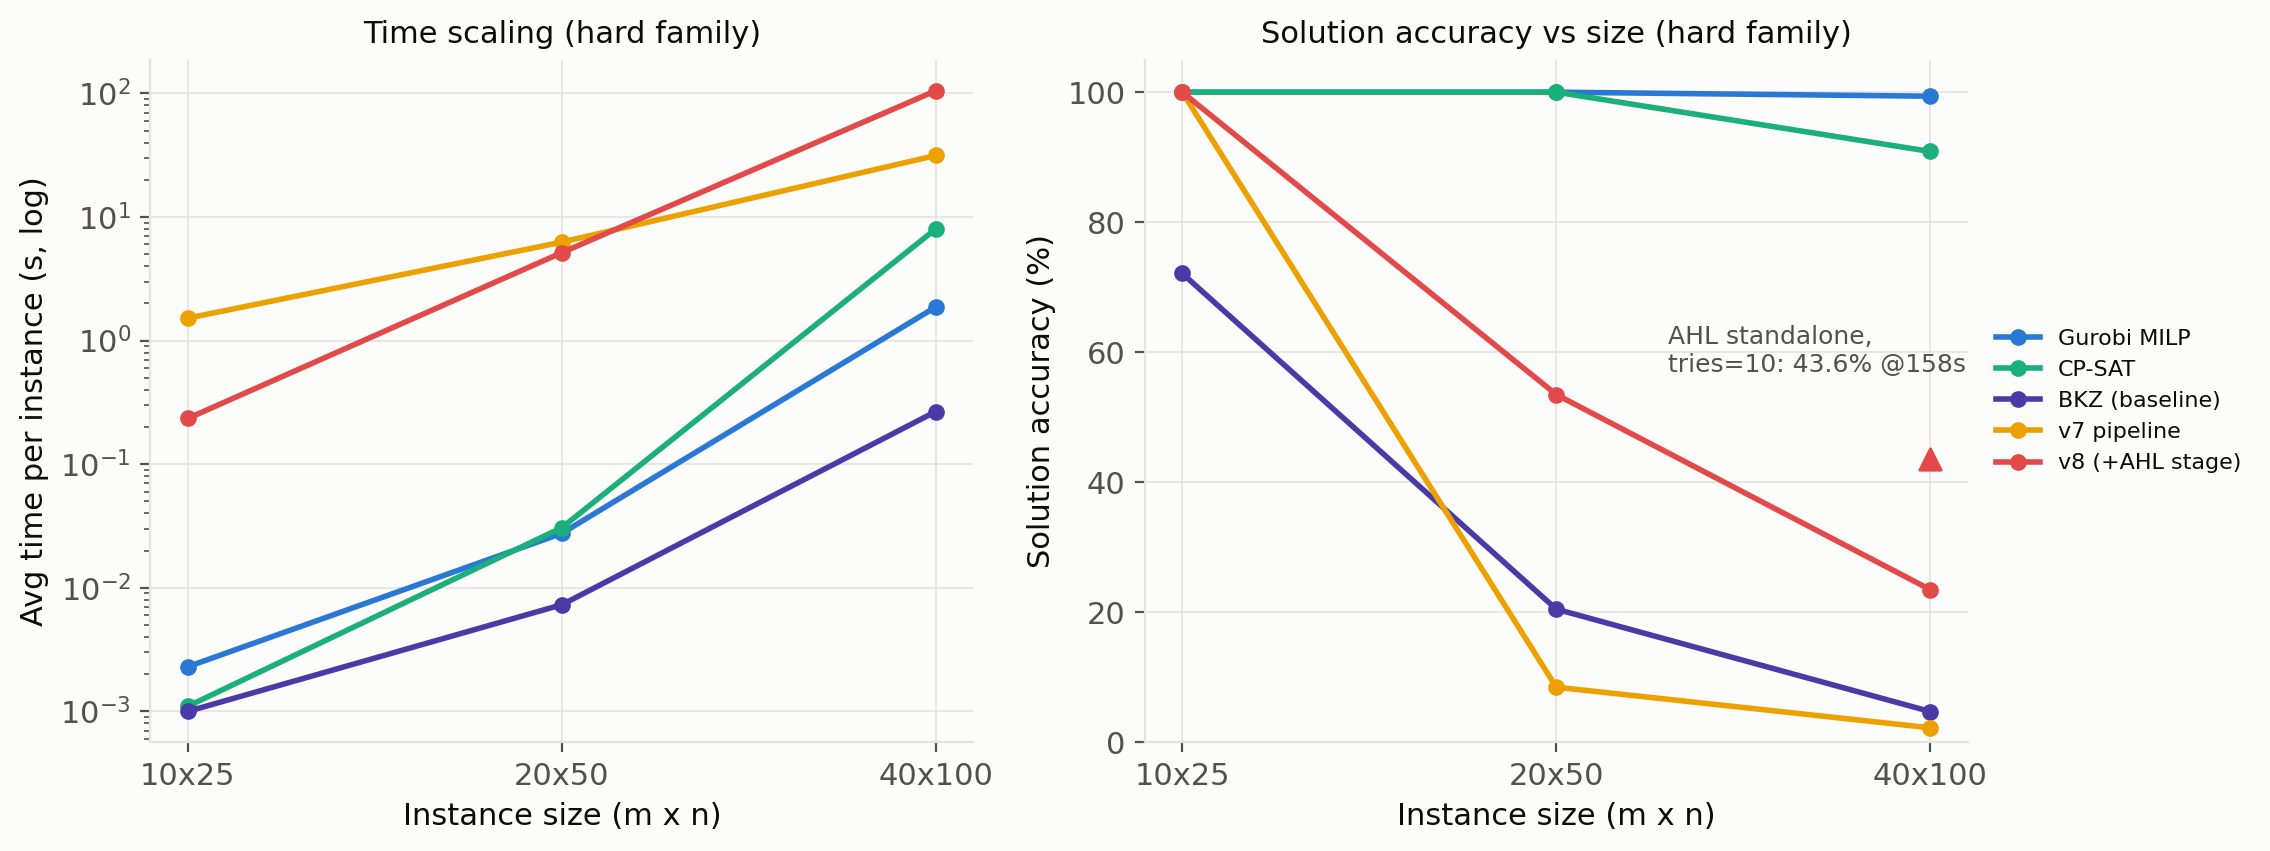
\includegraphics[width=\textwidth]{v8_scaling.png}
\caption{Time (log) and solution accuracy versus size. The triangle marks AHL standalone at ten tries (43.6\% at 158\,s), the anytime upper point of the v8 configuration shown as a line.}
\label{fig:v8}
\end{figure}

Three readings. First, v8 is now the strongest inexact method at every size: at $20 \times 50$ it solves 2.6$\times$ the best lattice baseline's share (53.5\% vs.\ 20.5\%) with zero false negatives, and at $40 \times 100$ it exceeds the baseline by 4.9--9$\times$ depending on the AHL budget (23.5\% at four tries, 43.6\% at ten). Second, the AHL stage also \emph{accelerates} the easy regime: at $10 \times 25$ it absorbs 533 of 1{,}000 instances in milliseconds (the remainder resolve through the pump and search stages as before), cutting mean time 6.5$\times$ at unchanged 100\% solution accuracy (feasibility dips from 100\% to 99.4\% because this evaluation used the pre-trained rather than the imitation checkpoint; the v7 report's per-role checkpoint recommendation stands). Third, exact solvers remain ahead wherever they finish within limits; the honest position is unchanged --- the pipeline's case rests on the sizes beyond $40 \times 100$ where their runtime explosion continues, and its zero-false-negative profile.

\section{Consequences for the Learned Components}

The search-technology question that blocked two cycles is now settled empirically: dense BLS yields to basis reduction, not to conflict learning or box-pruned enumeration. This reframes where learning can contribute next: (i) \emph{try scheduling} --- the AHL median-tries-to-hit is two, and unsolved instances burn the full try budget, so a learned predictor of "reducible now vs.\ needs another permutation" or a learned permutation proposal could cut the dominant cost at $40 \times 100$ several-fold; (ii) \emph{budget allocation} --- a hardness regressor routing instances between the millisecond stages and the expensive AHL/search tail; (iii) the fail-first ordering result of v7 continues to apply to the DFS proof side. These are measurement-backed, bounded roles, unlike the open-loop policy training that three independent attempts have now retired.

\begin{thebibliography}{9}
\bibitem[Aardal et al.(2000)]{aardal2000market}
Aardal, K., Bixby, R. E., Hurkens, C. A. J., Lenstra, A. K., \& Smeltink, J. W. (2000). Market split and basis reduction: Towards a solution of the Cornu\'ejols--Dawande instances. \emph{INFORMS Journal on Computing, 12}(3), 192--202.

\bibitem[Schnorr \& Euchner(1994)]{schnorr1994lattice}
Schnorr, C. P., \& Euchner, M. (1994). Lattice basis reduction: Improved practical algorithms and solving subset sum problems. \emph{Mathematical Programming, 66}(1--3), 181--199.
\end{thebibliography}

\end{document}
